\documentclass[professionalfont]{beamer}

\usepackage[T1]{fontenc}
\usepackage{amsmath}
\usepackage{graphicx}
\graphicspath{{figures/}}
\usepackage{tikz}
 
% usage: \tikzpic{<x percent>}{<y percent>}{<image size>}{<image name>}
\newcommand*{\tikzpic}[4]{%
\begin{tikzpicture}[remember picture,overlay]
\node at (current page.south west) [xshift=#1\paperwidth,yshift=#2\paperheight] {\includegraphics[width=#3\linewidth]{#4}};
\end{tikzpicture}%
}

\title[Gene expression inference with Deep Learning]{\textbf{\\Gene expression inference\\ with Deep Learning}}
\author[A. Sessa]{\underline{Andrea Sessa}\\
\vspace{2mm}
{\small \href{mailto:andrea.sessa@mail.polimi.it}{\nolinkurl{andrea.sessa@mail.polimi.it}}}\\
 \small{Yifei Chen, Yi Li, Rajiv Narayan, \\ Aravind Subramanian, Xiaohui Xie} \\
 \small{Bioinformatics, 2016 \\ Volume 32, Issue 12, pages: 1832-1839}}
\date{}

\usetheme{POLIMI}

\expandafter\def\expandafter\insertshorttitle\expandafter{\insertshorttitle\hfill\insertframenumber\,/\,\inserttotalframenumber}

\begin{document}

  \begin{frame}[plain]
    \titlepage
  \end{frame}

  \begin{frame}{Table of contents}
    \tableofcontents
  \end{frame}

  \begin{frame}{block}
    \begin{block}{title}
      bla bla bla
    \end{block}
  \end{frame}

  \section{Introduction}
  
    \subsection{Motivations}
      \begin{frame}
	\frametitle{Motivations}
	  \begin{itemize}
	   \item A fundamental problem in molecular biology: Characterize gene expression pattern under certain biological states
	   \item \textbf{Gene expression profiling} has been historically used as a tool to capture the gene expression patterns in response to \textbf{diseases}
	   \item Unfortunately, whole-genome gene expression profiling is still \textbf{too expensive} to be used in a typical academic lab to
		 generate a compendium over thousand of samples
           \item Human genome: $\sim 21000$ genes!
	  \end{itemize}
      \end{frame}

    \subsection{Previous Works}
      \begin{frame}
	\frametitle{Previous Works}
	  \begin{itemize}
	   \item \textbf{Main idea}: The expression profile of genes are known to be \textbf{highly} correlated!  
	   \item \textbf{C}onnectivity \textbf{MAP}: Creation of a large reference collection gene expression patterns of the human genome
	   \item \textbf{LINCS}: PCA analysis over the CMAP data; only $\sim 1000$ genes of 21000 capture the 80\% of the variance!
	     \begin{itemize}
	      \item The chosen 1000 genes are called \textbf{landmark genes}
	      \item The remaining part are called \textbf{target genes}
	      \item Measure gene expression of the landmark genes under certain biological condition(low cost!)
	      \item Infer the expression of the target genes from the landmark genes and other expression profile
	      \item LINCS program currently use \textbf{linear regression} to infer the expression of the target genes
	     \end{itemize}
	 \end{itemize}
      \end{frame}

    \section{Formalization}
      
      \subsection{Problem Statement}
	\begin{frame}
	 \frametitle{Problem Statement}
	 \begin{itemize}
	  \item Computationally complex to infer the expression profiles of target genes based on landmark genes
	  \item A large-scale multi-task machine learning problem!
	  \item We need also to consider that the target dimension(21000) is significantly \textbf{greater} thant the feature dimension(1000)
	  \begin{itemize}
	    \item LINCS uses linear regression, high scalability but it ignores \textbf{non-linearity patterns} inside the data
	    \item Others(\textit{Ye et al. 2006}) have tried to use kernel machines(ie. SVM), scalability problem!
	    \item Seems natural to adopt \textbf{Deep Learning} approach, high scalability + high representability 
	  \end{itemize}
	 \end{itemize}
	\end{frame}


      \subsection{Deep Learning Architecture}
	\begin{frame}
	  Idea: learn a \textbf{hierarchical} rappresentation of the data through multiple layers
	  \frametitle{Deep Learning Architecture}
	  \begin{center}
	    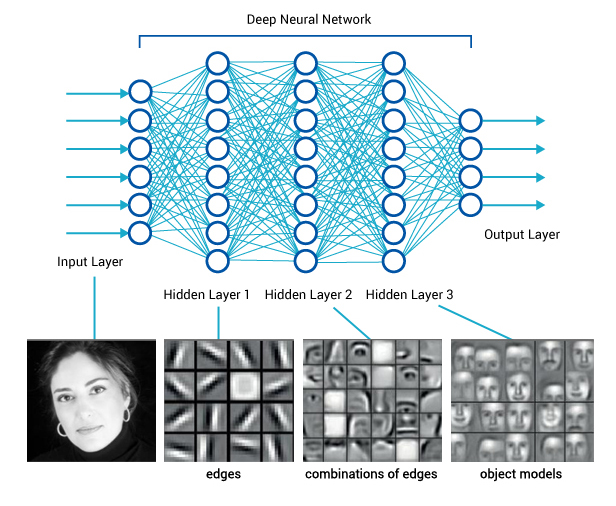
\includegraphics[scale=0.35]{deep_learning_net.jpg}
	  \end{center}
	\end{frame}

      \subsection{Linear Regression}
	\begin{frame}
	  \frametitle{Linear Regression}
	  \POLIMItitle{POLIMI Title}
	\end{frame}

      \subsection{KNN}
	\begin{frame}
	  \frametitle{KNN}
	  \POLIMItitle{POLIMI Title}
	\end{frame}

      \subsection{Datasets}
	\begin{frame}
	  \frametitle{Datasets}
	  \POLIMItitle{POLIMI Title}
	\end{frame}

      \subsection{D-GEX}
	\begin{frame}
	  \frametitle{D-GEX}
	  \POLIMItitle{POLIMI Title}
	\end{frame}

  \section{Results and Interpretation}

    \subsection{D-GEX Results}
      \begin{frame}
	\frametitle{D-GEX Results}
	\POLIMItitle{POLIMI Title}
      \end{frame}

    \subsection{Network Interpretation}
      \begin{frame}
	\frametitle{Network Interpretation}
	\POLIMItitle{POLIMI Title}
      \end{frame}
    
\end{document}
